\documentclass[border=10pt]{standalone}

\usepackage{tikz}
\usepackage{tikzsymbols}
\usetikzlibrary{calc,patterns,shapes.geometric}

\def\centerarc[#1](#2)(#3:#4:#5){\draw[#1] ($(#2)+({#5*cos(#3)},{#5*sin(#3)})$) arc (#3:#4:#5);}

\begin{document}
	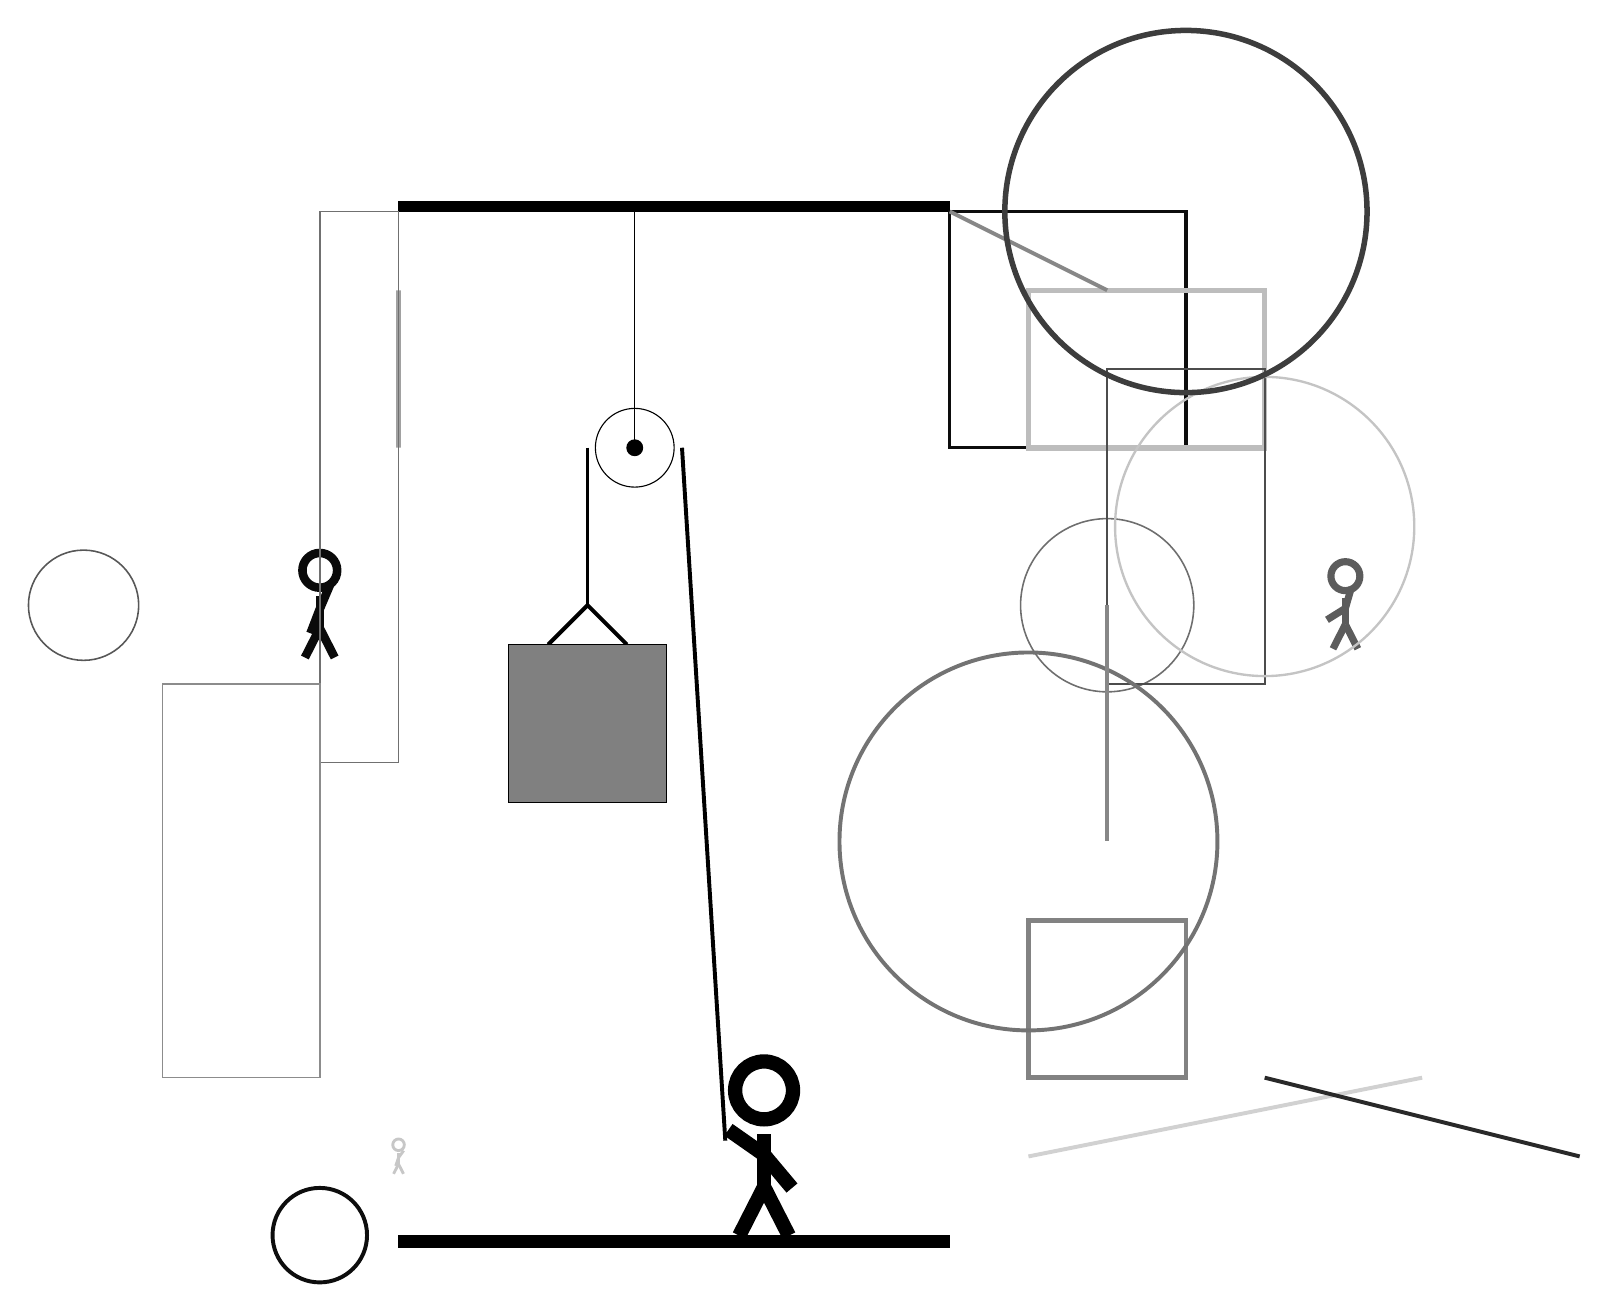
\begin{tikzpicture}
		%%%%% START %%%%%
		
		\draw[fill=black] (-2, 10) rectangle (5, 10.125);
		
		\draw (1, 7) circle (0.5);
		\draw[fill=black] (1, 7) circle (0.1);
		\draw (1, 10) -- (1, 7);
		
		\draw[line width=0.5mm] (-0.1, 4.5) -- (0.4, 5.0) -- (0.9, 4.5);
		\draw[fill=black!50] (-0.6, 4.5) rectangle (1.4, 2.5);
		
		\draw[line width=0.5mm] (0.4, 7) -- (0.4, 5.0);
		\centerarc[line width=0.5mm](1, 7)(0:180:0.6);
		\draw[line width=0.5mm](1.6, 7) -- (2.15, -1.8);
		
		\node at (2.6, -1.9) {\Strichmaxerl[10][-35][-50]};
		
		\draw[line width=0.4mm, color=black!95] (5, 10) rectangle (8, 7);
		
		\node[line width=0.5mm, color=black!22] at (-2, -2) {\Strichmaxerl[2][71][54]};
		\draw[line width=0.5mm, color=black!18](6, -2) -- (11, -1);
		\draw[line width=0.7mm, color=black!37] (-2, 9) rectangle (-2, 7);
		\node[line width=0.3mm, color=black!96] at (-3, 5) {\Strichmaxerl[6][69][67]};
		\draw [line width=0.2mm, color=black!57](7, 5) circle (1.1);
		\draw[line width=0.7mm, color=black!26] (6, 7) rectangle (9, 9);
		\draw[line width=0.5mm, color=black!47](7, 9) -- (5, 10);
		\draw[line width=0.6mm, color=black!49] (6, -1) rectangle (8, 1);
		\draw[line width=0.2mm, color=black!56] (-2, 3) rectangle (-3, 10);
		\node[line width=0.2mm, color=black!64] at (10, 5) {\Strichmaxerl[5][32][74]};
		\draw[line width=0.3mm, color=black!70] (7, 8) rectangle (9, 4);
		\draw [line width=0.5mm, color=black!55](6, 2) circle (2.4);
		\draw[line width=0.2mm, color=black!45] (-3, 4) rectangle (-5, -1);
		\draw [line width=0.3mm, color=black!23](9, 6) circle (1.9);
		\draw [line width=0.7mm, color=black!76](8, 10) circle (2.3);
		
		\draw [line width=0.5mm, color=black!95](-3, -3) circle (0.6);
		
		\draw [line width=0.2mm, color=black!66](-6, 5) circle (0.7);
		\draw[line width=0.5mm, color=black!47](7, 5) -- (7, 2);
		\draw[line width=0.5mm, color=black!84](9, -1) -- (13, -2);
		
		\draw[fill=black] (-2, -3) rectangle (5, -3.15);
		
		%%%%% END %%%%%
	\end{tikzpicture}
\end{document}